\documentclass[spanish,a4paper,11pt,twoside]{report}

%%%%%%%%%%%%%%%%%%%%%%%%%%%%%%%%%%%%%%%%%%%%%%%%%%%%%%%%%%%%%%%%%%%%%%%%%%%%%%%
\usepackage[dvips]{graphicx}
\usepackage[dvips]{epsfig}
\usepackage[latin1]{inputenc}
\usepackage[spanish]{babel}
\usepackage{alltt}
%\usepackage{templates/algorithm}
%\usepackage{templates/algorithmic}
%\usepackage{templates/multirow}

%%%%%%%%%%%%%%%%%%%%%%%%%%%%%%%%%%%%%%%%%%%%%%%%%%%%%%%%%%%%%%%%%%%%%%%%%%%%%%%

\newcommand{\SONY}{{\sc Sony}}
\newcommand{\MICROSOFT}{{\sc Microsoft}}
\newcommand{\GCC}{\textsf{\textsc{G}CC}}
\newcommand{\INTEL}{\textsf{\textsc{I}ntel}}

%%% Traducimos el pseudocodigo
%\renewcommand{\algorithmicwhile}{\textbf{mientras}}
%\renewcommand{\algorithmicend}{\textbf{fin}}
%\renewcommand{\algorithmicdo}{\textbf{hacer}}
%\renewcommand{\algorithmicif}{\textbf{si}}
%\renewcommand{\algorithmicthen}{\textbf{entonces}}
%\renewcommand{\algorithmicrepeat}{\textbf{repetir}}
%\renewcommand{\algorithmicuntil}{\textbf{hasta que}}
%\renewcommand{\algorithmicelse}{\textbf{en otro caso}}
%\renewcommand{\algorithmicfor}{\textbf{para}}

%\newcommand{\RETURN}{\textbf{retornar} }
\newcommand{\RET}{\STATE \textbf{retornar} }
\newcommand{\TO}{\textbf{hasta} }
\newcommand{\AND}{\textbf{y} }
\newcommand{\OR}{\textbf{o} }

%%%%%%%%%%%%%%%%% Creamos un entorno para listar c�digo fuente %%%%%%%%%%%%%%%
\newenvironment{sourcecode}
{\begin{list}{}{\setlength{\leftmargin}{1em}}\item\scriptsize\bfseries}
{\end{list}}

\newenvironment{littlesourcecode}
{\begin{list}{}{\setlength{\leftmargin}{1em}}\item\tiny\bfseries}
{\end{list}}

\newenvironment{summary}
{\par\noindent\begin{center}\textbf{Abstract}\end{center}\begin{itshape}\par\noindent}
{\end{itshape}}

\newenvironment{keywords}
{\begin{list}{}{\setlength{\leftmargin}{1em}}\item[\hskip\labelsep \bfseries Keywords:]}
{\end{list}}

\newenvironment{palabrasClave}
{\begin{list}{}{\setlength{\leftmargin}{1em}}\item[\hskip\labelsep \bfseries Palabras clave:]}
{\end{list}}


%%%%%%%%%%%%%%%%%%%%%%%%%%%%%%%%%%%%%%%%%%%%%%%%%%%%%%%%%%%%%%%%%%%%%%%%%%%%%%%
% Format
%%%%%%%%%%%%%%%%%%%%%%%%%%%%%%%%%%%%%%%%%%%%%%%%%%%%%%%%%%%%%%%%%%%%%%%%%%%%%%%

%%\topmargin -4 mm
%\topmargin -21 mm
%\headheight 10 mm
%\headsep 10 mm

%\textheight 229 mm
%\textheight 246 mm

%\oddsidemargin -5.4 mm
%\evensidemargin -5.4 mm
\oddsidemargin 5 mm
\evensidemargin 5 mm

%\oddsidemargin -3 mm
%\evensidemargin -3 mm

%\textwidth 17 cm
\textwidth 15 cm
%\columnsep 10 mm

\input{amssym.def}

%%%%%%%%%%%%%%%%%%%%%%%%%%%%%%%%%%%%%%%%%%%%%%%%%%%%%%%%%%%%%%%%%%%%%%%%%%%%%%%

\begin{document}

%%%%%%%%%%%%%%%%%%%%%%%%%%%%%%%%%%%%%%%%%%%%%%%%%%%%%%%%%%%%%%%%%%%%%%%%%%%%%%%
% First Page 
%%%%%%%%%%%%%%%%%%%%%%%%%%%%%%%%%%%%%%%%%%%%%%%%%%%%%%%%%%%%%%%%%%%%%%%%%%%%%%%

\pagestyle{empty}
\thispagestyle{empty}


\newcommand{\HRule}{\rule{\linewidth}{1mm}}
\setlength{\parindent}{0mm}
\setlength{\parskip}{0mm}
\vspace*{\stretch{1}}

\begin{center}

\includegraphics[width=0.2\textwidth]{./img/logotipo-secundario-ULL}\\[0.25cm]
\end{center}

\HRule
\begin{center}
        {\Huge Integraci�n Trapecio} \\[2.5mm] 
        {\Huge $f(x)=sen(\Pi x)$, $x \in [-2,-1]$} \\[2.5mm]
        {\Large  Lara Kristjansdottir, Javier Hern�ndez P�rez} \\[5mm]
        {\Large \textit{Grupo ($2\mid F$) }} \\[5mm]


        {\em T�cnicas Experimentales. $1^{er}$ curso. $2^{do}$ semestre} \\[5mm]
        Lenguajes y Sistemas Inform�ticos \\[5mm]
        Facultad de Matem�ticas \\[5mm]
        
        Universidad de La Laguna \\
\end{center}
\HRule
\vspace*{\stretch{2}}
\begin{center}
  La Laguna, \today 
\end{center}

%%%%%%%%%%%%%%%%%%%%%%%%%%%%%%%%%%%%%%%%%%%%%%%%%%%%%%%%%%%%%%%%%%%%%%%%%%%%%%%

%%%%%%%%%%%%%%%%%%%%%%%%%%%%%%%%%%%%%%%%%%%%%%%%%%%%%%%%%%%%%%%%%%%%%%%%%%%%%%%
\newpage{\pagestyle{empty}\cleardoublepage}

\pagestyle{myheadings} %my head defined by markboth or markright
% No funciona bien \markboth sin "twoside" en \documentclass, pero al
% ponerlo se dan un mont�n de errores de underfull \vbox, con lo que no se
% ha puesto.
\markboth{Lara Kristjansdottir, Javier Hern�ndez P�rez}{Integraci�n Trapecio $f(x)=sen(\Pi x)$, $x \in [-2,-1]$}

%%%%%%%%%%%%%%%%%%%%%%%%%%%%%%%%%%%%%%%%%%%%%%%%%%%%%%%%%%%%%%%%%%%%%%%%%%%%%%%
%Numeracion en romanos
\renewcommand{\thepage}{\roman{page}}
\setcounter{page}{1}

%%%%%%%%%%%%%%%%%%%%%%%%%%%%%%%%%%%%%%%%%%%%%%%%%%%%%%%%%%%%%%%%%%%%%%%%%%%%%%%

\tableofcontents

%%%%%%%%%%%%%%%%%%%%%%%%%%%%%%%%%%%%%%%%%%%%%%%%%%%%%%%%%%%%%%%%%%%%%%%%%%%%%%%
\newpage{\pagestyle{empty}\cleardoublepage}

\listoffigures

%%%%%%%%%%%%%%%%%%%%%%%%%%%%%%%%%%%%%%%%%%%%%%%%%%%%%%%%%%%%%%%%%%%%%%%%%%%%%%%
\newpage{\pagestyle{empty}\cleardoublepage}

\listoftables

%%%%%%%%%%%%%%%%%%%%%%%%%%%%%%%%%%%%%%%%%%%%%%%%%%%%%%%%%%%%%%%%%%%%%%%%%%%%%%%
\newpage{\pagestyle{empty}\cleardoublepage}

%%%%%%%%%%%%%%%%%%%%%%%%%%%%%%%%%%%%%%%%%%%%%%%%%%%%%%%%%%%%%%%%%%%%%%%%%%%%%%%
%Numeracion a partir del capitulo I
\renewcommand{\thepage}{\arabic{page}}
\setcounter{page}{1}

\setlength{\parindent}{5mm}

%%%%%%%%%%%%%%%%%%%%%%%%%%%%%%%%%%%%%%%%%%%%%%%%%%%%%%%%%%%%%%%%%%%%%%%%%%%%%%%
\chapter{Motivaci�n y objetivos}
\label{chapter:obj}

%%%%%%%%%%%%%%%%%%%%%%%%%%%%%%%%%%%%%%%%%%%%%%%%%%%%%%%%%%%%%%%%%%%%%%%%%%%%%
% Chapter 1: Motivaci�n y Objetivos 
%%%%%%%%%%%%%%%%%%%%%%%%%%%%%%%%%%%%%%%%%%%%%%%%%%%%%%%%%%%%%%%%%%%%%%%%%%%%%%%

%Los objetivos le dan al lector las razones por las que se realiz� el
%proyecto o trabajo de investigaci�n.
%---------------------------------------------------------------------------------
\section{Utilidad el m�todo}
\label{1:sec:1}
 % Primer p�rrafo de la primera secci�n.
No todas las integrales se pueden resolver por ello es muy importante el hecho de tener algunos m�todos que nos permitan aproximar las integrales cuando tenemos una integral definida. En este caso nos centraremos en el m�todo de los trapecios.\par

Adem�s este m�todo tiene una importancia extra. Si un m�todo, como este, es sencillo.Teniendo en cuenta que con funciones en la vida real, midiendo un terreno por ejemplo,normalmente (salvo casos particulares como por ejemplo una persona con un terreno cuadrado que quiera que cada uno de sus dos hijos hereden la mitad de su terreno dividido por la funci�n $sen(\pi x)$) estas haciendo una aproximaci�n.Usar directamente el m�todo de los trapecios parece una opci�n l�gica.\par

Por ejemplo hallas el �rea de un cuadrado al medio del terreno y vas eligiendo puntos de la frontera del terreno que esten unidos aproximadamente por lineas rectas. Ya solo queda hallar el area de los trapecios con base el lado del cuadrado que les quede m�s cerca y sumar.
%---------------------------------------------------------------------------------
\section{Nuestra integral $f(x)=sen(\pi x)$, $x \in [-2,-1]$ se puede resolver}
\label{1:sec:2}
  %Primer p�rrafo de la segunda secci�n.
  Nuestra integral es facil resolverla, lo cual es una gran ventaja ya que nos permite comprobar. Lo r�pido que aproxima el m�todo de los trapecios, y la efectividad del ordenador con dicho m�todo. \par
  
  Resolvamos ahora $\int _{-2}^{-1}sen(\pi x)dx$. Haciendo el cambio $y=\pi x$ teniendo en cuenta que $\frac {\partial y} {\partial x}=\pi$ , $ x=-2 \Rightarrow y=-2 \cdot \pi$ , $ x=-1 \Rightarrow y=-\pi$ obtenemos que $\int _{-2}^{-1} sen(\pi x) dx=\frac{\int _{-2 \pi}^{-1\pi}sen(y)dy}{\pi}=\frac{-cos(-2 \cdot \pi)+cos(-\pi)}{\pi}=\frac{1-1}{\pi}=0$

\begin{itemize}
  \item Item 1
  \item Item 2
  \item Item 3
\end{itemize}



%%%%%%%%%%%%%%%%%%%%%%%%%%%%%%%%%%%%%%%%%%%%%%%%%%%%%%%%%%%%%%%%%%%%%%%%%%%%%%%
\chapter{Fundamentos te�ricos}
\label{chapter:teo}

%%%%%%%%%%%%%%%%%%%%%%%%%%%%%%%%%%%%%%%%%%%%%%%%%%%%%%%%%%%%%%%%%%%%%%%%%%%%%%%
% Chapter 2: Fundamentos Te�ricos 
%%%%%%%%%%%%%%%%%%%%%%%%%%%%%%%%%%%%%%%%%%%%%%%%%%%%%%%%%%%%%%%%%%%%%%%%%%%%%%%

%++++++++++++++++++++++++++++++++++++++++++++++++++++++++++++++++++++++++++++++

En este cap�tulo se han de presentar los antecedentes te�ricos y pr�cticos que
apoyan el tema objeto de la investigaci�n.

%++++++++++++++++++++++++++++++++++++++++++++++++++++++++++++++++++++++++++++++

\section{Primer apartado del segundo cap�tulo}
\label{2:sec:1}
  Primer p�rrafo de la primera secci�n.

\section{Segundo apartado del segundo cap�tulo}
\label{2:sec:2}
  Primer p�rrafo de la segunda secci�n.



%%%%%%%%%%%%%%%%%%%%%%%%%%%%%%%%%%%%%%%%%%%%%%%%%%%%%%%%%%%%%%%%%%%%%%%%%%%%%%%
\chapter{Procedimiento experimental}
\label{chapter:exp}

%%%%%%%%%%%%%%%%%%%%%%%%%%%%%%%%%%%%%%%%%%%%%%%%%%%%%%%%%%%%%%%%%%%%%%%%%%%%%%%
% Chapter 3: Procedimiento experimental 
%%%%%%%%%%%%%%%%%%%%%%%%%%%%%%%%%%%%%%%%%%%%%%%%%%%%%%%%%%%%%%%%%%%%%%%%%%%%%%%

%++++++++++++++++++++++++++++++++++++++++++++++++++++++++++++++++++++++++++++++
\section{Descripci�n de los experimentos}
\label{3:sec:1}

Vamos a aplicar la regla del trapecio a la funci�n sin(pi*x) en el intervalo [-2,-1] utilizando una cantidad variable de subintervalos, n. Para cada valor de n, mediremos el error absoluto y el tiempo de ejecuci�n del m�todo.

%++++++++++++++++++++++++++++++++++++++++++++++++++++++++++++++++++++++++++++++
\section{Descripci�n del material}
\label{3:sec:2}

Los experimentos han tenido lugar sobre un procesador Intel Core i3-2350M a 2.30 GHz. N�tese que aunque la m�quina tiene cuatro procesadores, s�lo se emple� uno para realizar los c�lculos. El sistema operativo fue Linux Mint 14.1 (Nadia) con la versi�n 3.5.0-17 del kernel. Los algoritmos fueron implementados en Python y la versi�n del int�rprete fue la 2.7.3.

%++++++++++++++++++++++++++++++++++++++++++++++++++++++++++++++++++++++++++++++
\section{Resultados obtenidos}
\label{3:sec:3}

Aqu� vamos a esperar hasta tener la tabla resumen, las gr�ficas y el c�lculo anal�tico de la cota del error.
%------------------------------------------------------------------------------
\begin{figure}[!th]
\begin{center}
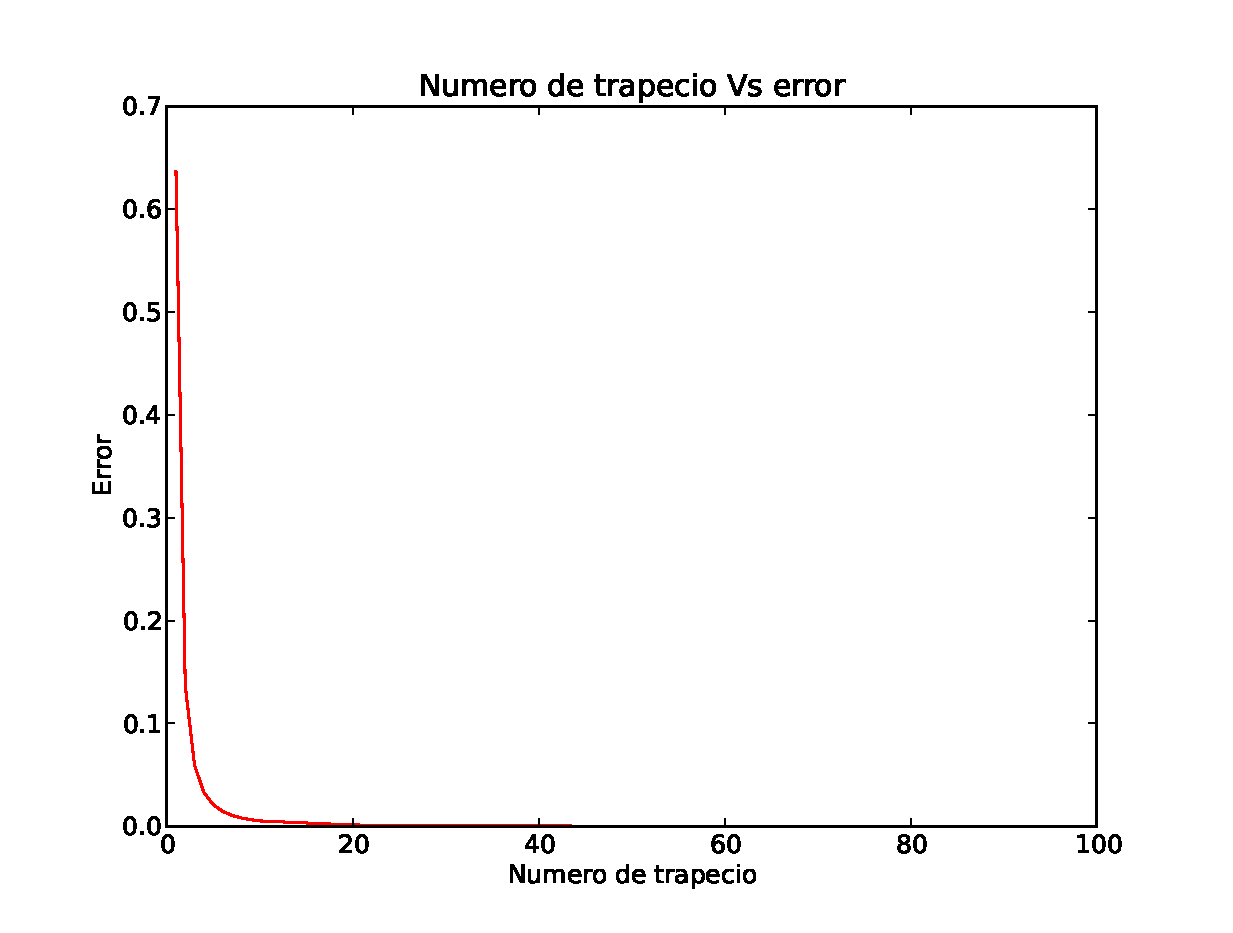
\includegraphics[width=0.75\textwidth]{img/Plot_nVSerror.eps}
\caption{nVSerror}
\label{fig:1}
\end{center}
\end{figure}
%------------------------------------------------------------------------------
\begin{figure}[!bh]
\begin{center}
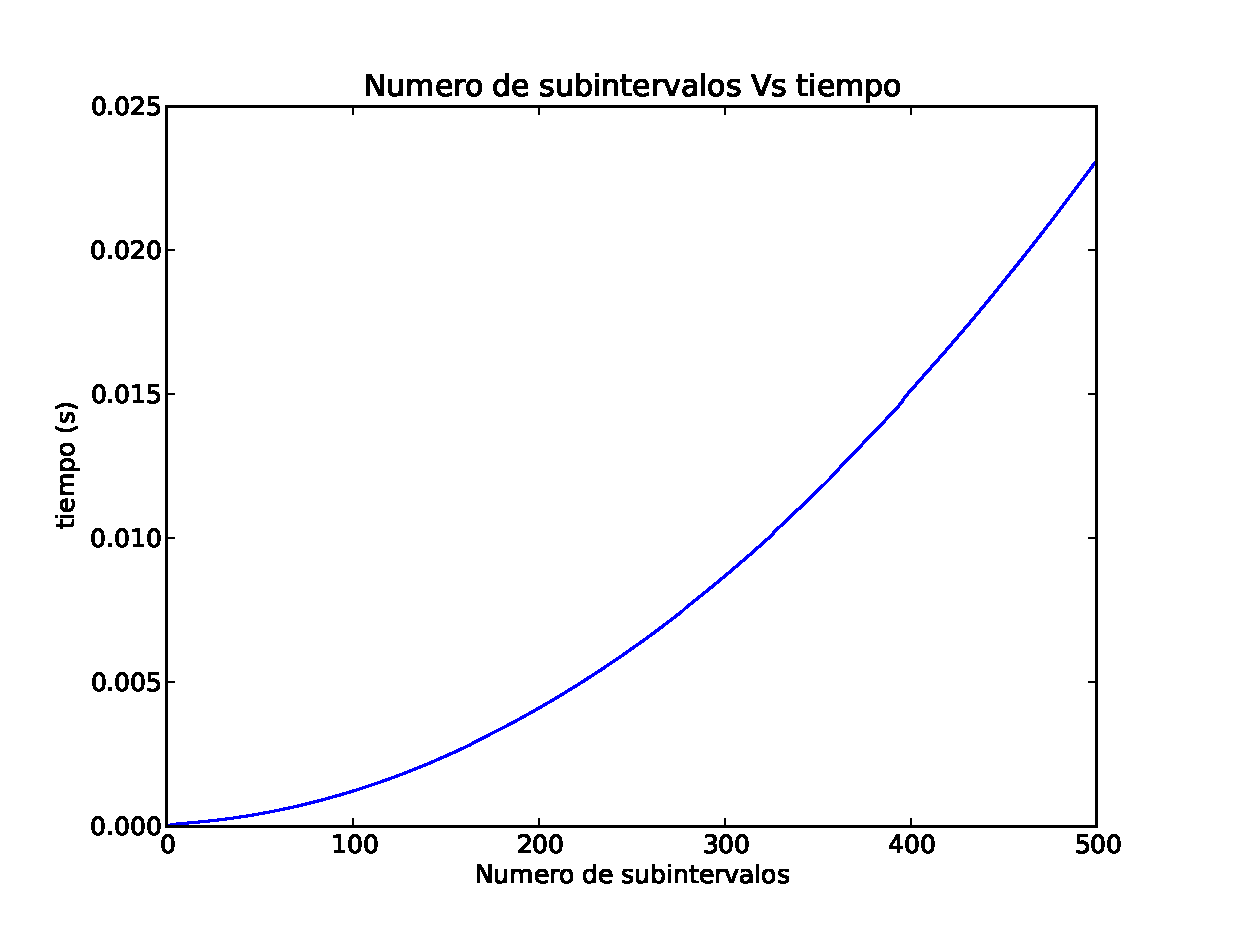
\includegraphics[width=0.75\textwidth]{img/Plot_nVStime.eps}
\caption{nVStiempo}
\label{fig:2}
\end{center}
\end{figure}
%------------------------------------------------------------------------------

\DTLloaddb[noheader,keys={n,error,tiempo}]{table1}{mydata.csv}
\newcolumntype{d}{D{,}{\pm}{-1}} 

\begin{table}[!h]
 \begin{center}
  \begin{tabular}{l|c|r}% 
    {\bf n} & {\bf error} & {\bf tiempo}
    \DTLforeach*{table1}{%
      \n=n,\error=error,\tiempo=tiempo}{%
      \\
      \n & \error & \tiempo}%
  \end{tabular}
  \caption{Resultados optenidos por número de trapecios}
  \label{tabla:1}
  \end{center}
\end{table}                                     

%------------------------------------------------------------------------------


%++++++++++++++++++++++++++++++++++++++++++++++++++++++++++++++++++++++++++++++
\section{An�lisis de los resultados}
\label{3:sec:4}

bla, bla, etc. 



%%%%%%%%%%%%%%%%%%%%%%%%%%%%%%%%%%%%%%%%%%%%%%%%%%%%%%%%%%%%%%%%%%%%%%%%%%%%%%%
\chapter{Conclusiones}
\label{chapter:conclusiones}

%%%%%%%%%%%%%%%%%%%%%%%%%%%%%%%%%%%%%%%%%%%%%%%%%%%%%%%%%%%%%%%%%%%%%%%%%%%%%
% Chapter 4: Conclusiones y Trabajos Futuros 
%%%%%%%%%%%%%%%%%%%%%%%%%%%%%%%%%%%%%%%%%%%%%%%%%%%%%%%%%%%%%%%%%%%%%%%%%%%%%%%
\section{Conclusiones}
\label{4:sec:1}
El m\'etodo del trapecio nos da una buena aproximaci\'on de la integral que quer\'iamos calcular con un coste temporal razonable. El error obtenido nunca supera la cota calculada y con m\'as subintervalos el error absoluto disminuye y la aproximaci\'on es m\'as precisa aunque se tarde m\'as.


%%%%%%%%%%%%%%%%%%%%%%%%%%%%%%%%%%%%%%%%%%%%%%%%%%%%%%%%%%%%%%%%%%%%%%%%%%%%%%%

%%%%%%%%%%%%%%%%%%%%%%%%%%%%%%%%%%%%%%%%%%%%%%%%%%%%%%%%%%%%%%%%%%%%%%%%%%%%%%%
\newpage{\pagestyle{empty}\cleardoublepage}
\thispagestyle{empty}
\begin{appendix}

\chapter{T�tulo del Ap�ndice 1}
\label{appendix:1}

\section{Algoritmo XXX}
\label{Apendice1:XXX}

\begin{center}
\begin{footnotesize}
\begin{verbatim}
###################################################################################
# Fichero .py
###################################################################################
#
# AUTORES
#   
# FECHA
#
# DESCRIPCION
#
###################################################################################
\end{verbatim}
\end{footnotesize}
\end{center}

\section{Algoritmo YYY}
\label{Apendice1:YYY}

\begin{center}
\begin{footnotesize}
\begin{verbatim}
/###################################################################################
 # Fichero .h
 ###################################################################################
 #
 # AUTORES
 #
 # FECHA
 #
 # DESCRIPCION
 #
 ##################################################################################
\end{verbatim}
\end{footnotesize}
\end{center}


\chapter{T�tulo del Ap�ndice 2}
\label{appendix:2}

\section{Otro apendice: Seccion 1}
\label{Apendice2:label}

\begin{center}
\begin{footnotesize}

\begin{verbatim}
Texto
\end{verbatim}

\end{footnotesize}
\end{center}

\section{Otro apendice: Seccion 2}
\label{Apendice2:label2}

\begin{center}
\begin{footnotesize}

\begin{verbatim}
Texto
\end{verbatim}


\end{footnotesize}
\end{center}


\end{appendix}

%%%%%%%%%%%%%%%%%%%%%%%%%%%%%%%%%%%%%%%%%%%%%%%%%%%%%%%%%%%%%%%%%%%%%%%%%%%%%%%
\addcontentsline{toc}{chapter}{Bibliograf�a}
\bibliographystyle{plain}


\bibliography{bib/references}
\nocite{*}

%%%%%%%%%%%%%%%%%%%%%%%%%%%%%%%%%%%%%%%%%%%%%%%%%%%%%%%%%%%%%%%%%%%%%%%%%%%%%%%

\end{document}
